% !TEX TS-program = pdflatex
% !TEX encoding = UTF-8 Unicode
\documentclass[border=0mm]{standalone}
% packages
\usepackage{tikz}
\usetikzlibrary{patterns}
\usepackage{amsmath,amssymb}
\usepackage{bm}
\usepackage{pgfplots}
\pgfplotsset{compat=1.15}
% start document
\begin{document}
% generated by ROOT (CERN)
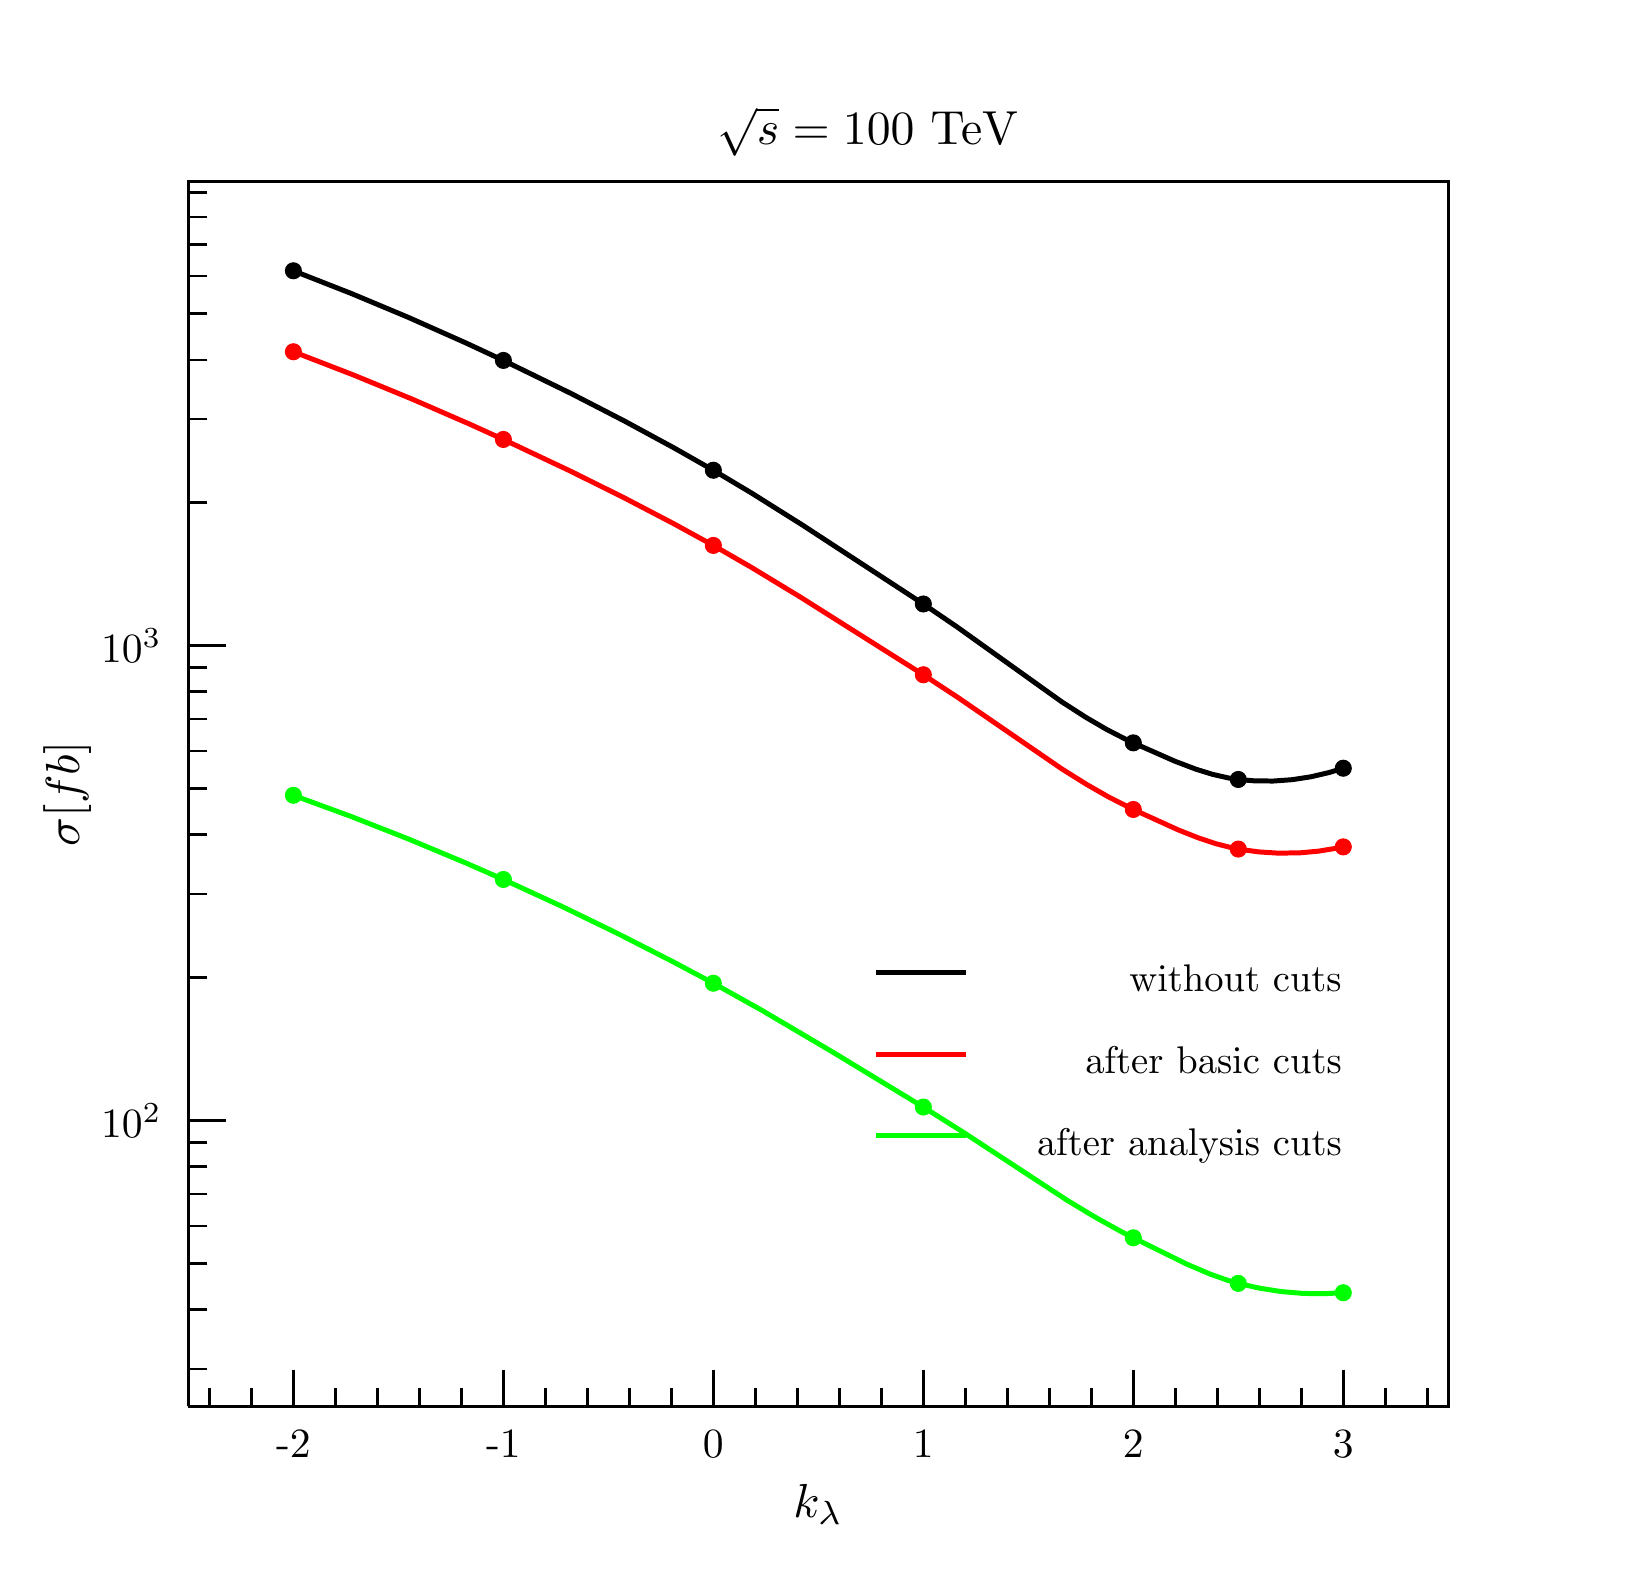
\begin{tikzpicture}
\pgfdeclareplotmark{cross} {
\pgfpathmoveto{\pgfpoint{-0.3\pgfplotmarksize}{\pgfplotmarksize}}
\pgfpathlineto{\pgfpoint{+0.3\pgfplotmarksize}{\pgfplotmarksize}}
\pgfpathlineto{\pgfpoint{+0.3\pgfplotmarksize}{0.3\pgfplotmarksize}}
\pgfpathlineto{\pgfpoint{+1\pgfplotmarksize}{0.3\pgfplotmarksize}}
\pgfpathlineto{\pgfpoint{+1\pgfplotmarksize}{-0.3\pgfplotmarksize}}
\pgfpathlineto{\pgfpoint{+0.3\pgfplotmarksize}{-0.3\pgfplotmarksize}}
\pgfpathlineto{\pgfpoint{+0.3\pgfplotmarksize}{-1.\pgfplotmarksize}}
\pgfpathlineto{\pgfpoint{-0.3\pgfplotmarksize}{-1.\pgfplotmarksize}}
\pgfpathlineto{\pgfpoint{-0.3\pgfplotmarksize}{-0.3\pgfplotmarksize}}
\pgfpathlineto{\pgfpoint{-1.\pgfplotmarksize}{-0.3\pgfplotmarksize}}
\pgfpathlineto{\pgfpoint{-1.\pgfplotmarksize}{0.3\pgfplotmarksize}}
\pgfpathlineto{\pgfpoint{-0.3\pgfplotmarksize}{0.3\pgfplotmarksize}}
\pgfpathclose
\pgfusepathqstroke
}
\pgfdeclareplotmark{cross*} {
\pgfpathmoveto{\pgfpoint{-0.3\pgfplotmarksize}{\pgfplotmarksize}}
\pgfpathlineto{\pgfpoint{+0.3\pgfplotmarksize}{\pgfplotmarksize}}
\pgfpathlineto{\pgfpoint{+0.3\pgfplotmarksize}{0.3\pgfplotmarksize}}
\pgfpathlineto{\pgfpoint{+1\pgfplotmarksize}{0.3\pgfplotmarksize}}
\pgfpathlineto{\pgfpoint{+1\pgfplotmarksize}{-0.3\pgfplotmarksize}}
\pgfpathlineto{\pgfpoint{+0.3\pgfplotmarksize}{-0.3\pgfplotmarksize}}
\pgfpathlineto{\pgfpoint{+0.3\pgfplotmarksize}{-1.\pgfplotmarksize}}
\pgfpathlineto{\pgfpoint{-0.3\pgfplotmarksize}{-1.\pgfplotmarksize}}
\pgfpathlineto{\pgfpoint{-0.3\pgfplotmarksize}{-0.3\pgfplotmarksize}}
\pgfpathlineto{\pgfpoint{-1.\pgfplotmarksize}{-0.3\pgfplotmarksize}}
\pgfpathlineto{\pgfpoint{-1.\pgfplotmarksize}{0.3\pgfplotmarksize}}
\pgfpathlineto{\pgfpoint{-0.3\pgfplotmarksize}{0.3\pgfplotmarksize}}
\pgfpathclose
\pgfusepathqfillstroke
}
\pgfdeclareplotmark{newstar} {
\pgfpathmoveto{\pgfqpoint{0pt}{\pgfplotmarksize}}
\pgfpathlineto{\pgfqpointpolar{44}{0.5\pgfplotmarksize}}
\pgfpathlineto{\pgfqpointpolar{18}{\pgfplotmarksize}}
\pgfpathlineto{\pgfqpointpolar{-20}{0.5\pgfplotmarksize}}
\pgfpathlineto{\pgfqpointpolar{-54}{\pgfplotmarksize}}
\pgfpathlineto{\pgfqpointpolar{-90}{0.5\pgfplotmarksize}}
\pgfpathlineto{\pgfqpointpolar{234}{\pgfplotmarksize}}
\pgfpathlineto{\pgfqpointpolar{198}{0.5\pgfplotmarksize}}
\pgfpathlineto{\pgfqpointpolar{162}{\pgfplotmarksize}}
\pgfpathlineto{\pgfqpointpolar{134}{0.5\pgfplotmarksize}}
\pgfpathclose
\pgfusepathqstroke
}
\pgfdeclareplotmark{newstar*} {
\pgfpathmoveto{\pgfqpoint{0pt}{\pgfplotmarksize}}
\pgfpathlineto{\pgfqpointpolar{44}{0.5\pgfplotmarksize}}
\pgfpathlineto{\pgfqpointpolar{18}{\pgfplotmarksize}}
\pgfpathlineto{\pgfqpointpolar{-20}{0.5\pgfplotmarksize}}
\pgfpathlineto{\pgfqpointpolar{-54}{\pgfplotmarksize}}
\pgfpathlineto{\pgfqpointpolar{-90}{0.5\pgfplotmarksize}}
\pgfpathlineto{\pgfqpointpolar{234}{\pgfplotmarksize}}
\pgfpathlineto{\pgfqpointpolar{198}{0.5\pgfplotmarksize}}
\pgfpathlineto{\pgfqpointpolar{162}{\pgfplotmarksize}}
\pgfpathlineto{\pgfqpointpolar{134}{0.5\pgfplotmarksize}}
\pgfpathclose
\pgfusepathqfillstroke
}
\definecolor{c}{rgb}{1,1,1};
\draw [color=c, fill=c] (0,0) rectangle (20,19.4486);
\draw [color=c, fill=c] (0,0) rectangle (20,19.4486);
\draw [color=c, fill=c] (2,1.94486) rectangle (18,17.5038);
\definecolor{c}{rgb}{0,0,0};
\draw [c,line width=0.9] (2,1.94486) -- (2,17.5038) -- (18,17.5038) -- (18,1.94486) -- (2,1.94486);
\definecolor{c}{rgb}{1,1,1};
\draw [color=c, fill=c] (2,1.94486) rectangle (18,17.5038);
\definecolor{c}{rgb}{0,0,0};
\draw [c,line width=0.9] (2,1.94486) -- (2,17.5038) -- (18,17.5038) -- (18,1.94486) -- (2,1.94486);
\definecolor{c}{rgb}{0,0,0.6};
\draw [c,line width=0.9] (2,1.94486) -- (2.16,1.94486) -- (2.16,1.94486) -- (2.32,1.94486) -- (2.32,1.94486) -- (2.48,1.94486) -- (2.48,1.94486) -- (2.64,1.94486) -- (2.64,1.94486) -- (2.8,1.94486) -- (2.8,1.94486) -- (2.96,1.94486) -- (2.96,1.94486)
 -- (3.12,1.94486) -- (3.12,1.94486) -- (3.28,1.94486) -- (3.28,1.94486) -- (3.44,1.94486) -- (3.44,1.94486) -- (3.6,1.94486) -- (3.6,1.94486) -- (3.76,1.94486) -- (3.76,1.94486) -- (3.92,1.94486) -- (3.92,1.94486) -- (4.08,1.94486) -- (4.08,1.94486)
 -- (4.24,1.94486) -- (4.24,1.94486) -- (4.4,1.94486) -- (4.4,1.94486) -- (4.56,1.94486) -- (4.56,1.94486) -- (4.72,1.94486) -- (4.72,1.94486) -- (4.88,1.94486) -- (4.88,1.94486) -- (5.04,1.94486) -- (5.04,1.94486) -- (5.2,1.94486) -- (5.2,1.94486)
 -- (5.36,1.94486) -- (5.36,1.94486) -- (5.52,1.94486) -- (5.52,1.94486) -- (5.68,1.94486) -- (5.68,1.94486) -- (5.84,1.94486) -- (5.84,1.94486) -- (6,1.94486) -- (6,1.94486) -- (6.16,1.94486) -- (6.16,1.94486) -- (6.32,1.94486) -- (6.32,1.94486) --
 (6.48,1.94486) -- (6.48,1.94486) -- (6.64,1.94486) -- (6.64,1.94486) -- (6.8,1.94486) -- (6.8,1.94486) -- (6.96,1.94486) -- (6.96,1.94486) -- (7.12,1.94486) -- (7.12,1.94486) -- (7.28,1.94486) -- (7.28,1.94486) -- (7.44,1.94486) -- (7.44,1.94486) --
 (7.6,1.94486) -- (7.6,1.94486) -- (7.76,1.94486) -- (7.76,1.94486) -- (7.92,1.94486) -- (7.92,1.94486) -- (8.08,1.94486) -- (8.08,1.94486) -- (8.24,1.94486) -- (8.24,1.94486) -- (8.4,1.94486) -- (8.4,1.94486) -- (8.56,1.94486) -- (8.56,1.94486) --
 (8.72,1.94486) -- (8.72,1.94486) -- (8.88,1.94486) -- (8.88,1.94486) -- (9.04,1.94486) -- (9.04,1.94486) -- (9.2,1.94486) -- (9.2,1.94486) -- (9.36,1.94486) -- (9.36,1.94486) -- (9.52,1.94486) -- (9.52,1.94486) -- (9.68,1.94486) -- (9.68,1.94486) --
 (9.84,1.94486) -- (9.84,1.94486) -- (10,1.94486) -- (10,1.94486) -- (10.16,1.94486) -- (10.16,1.94486) -- (10.32,1.94486) -- (10.32,1.94486) -- (10.48,1.94486) -- (10.48,1.94486) -- (10.64,1.94486) -- (10.64,1.94486) -- (10.8,1.94486) --
 (10.8,1.94486) -- (10.96,1.94486) -- (10.96,1.94486) -- (11.12,1.94486) -- (11.12,1.94486) -- (11.28,1.94486) -- (11.28,1.94486) -- (11.44,1.94486) -- (11.44,1.94486) -- (11.6,1.94486) -- (11.6,1.94486) -- (11.76,1.94486) -- (11.76,1.94486) --
 (11.92,1.94486) -- (11.92,1.94486) -- (12.08,1.94486) -- (12.08,1.94486) -- (12.24,1.94486) -- (12.24,1.94486) -- (12.4,1.94486) -- (12.4,1.94486) -- (12.56,1.94486) -- (12.56,1.94486) -- (12.72,1.94486) -- (12.72,1.94486) -- (12.88,1.94486) --
 (12.88,1.94486) -- (13.04,1.94486) -- (13.04,1.94486) -- (13.2,1.94486) -- (13.2,1.94486) -- (13.36,1.94486) -- (13.36,1.94486) -- (13.52,1.94486) -- (13.52,1.94486) -- (13.68,1.94486) -- (13.68,1.94486) -- (13.84,1.94486) -- (13.84,1.94486) --
 (14,1.94486) -- (14,1.94486) -- (14.16,1.94486) -- (14.16,1.94486) -- (14.32,1.94486) -- (14.32,1.94486) -- (14.48,1.94486) -- (14.48,1.94486) -- (14.64,1.94486) -- (14.64,1.94486) -- (14.8,1.94486) -- (14.8,1.94486) -- (14.96,1.94486) --
 (14.96,1.94486) -- (15.12,1.94486) -- (15.12,1.94486) -- (15.28,1.94486) -- (15.28,1.94486) -- (15.44,1.94486) -- (15.44,1.94486) -- (15.6,1.94486) -- (15.6,1.94486) -- (15.76,1.94486) -- (15.76,1.94486) -- (15.92,1.94486) -- (15.92,1.94486) --
 (16.08,1.94486) -- (16.08,1.94486) -- (16.24,1.94486) -- (16.24,1.94486) -- (16.4,1.94486) -- (16.4,1.94486) -- (16.56,1.94486) -- (16.56,1.94486) -- (16.72,1.94486) -- (16.72,1.94486) -- (16.88,1.94486) -- (16.88,1.94486) -- (17.04,1.94486) --
 (17.04,1.94486) -- (17.2,1.94486) -- (17.2,1.94486) -- (17.36,1.94486) -- (17.36,1.94486) -- (17.52,1.94486) -- (17.52,1.94486) -- (17.68,1.94486) -- (17.68,1.94486) -- (17.84,1.94486) -- (17.84,1.94486) -- (18,1.94486);
\definecolor{c}{rgb}{0,0,0};
\draw [c,line width=0.9] (2,1.94486) -- (18,1.94486);
\draw [c,line width=0.9] (3.33333,2.41163) -- (3.33333,1.94486);
\draw [c,line width=0.9] (3.86667,2.17825) -- (3.86667,1.94486);
\draw [c,line width=0.9] (4.4,2.17825) -- (4.4,1.94486);
\draw [c,line width=0.9] (4.93333,2.17825) -- (4.93333,1.94486);
\draw [c,line width=0.9] (5.46667,2.17825) -- (5.46667,1.94486);
\draw [c,line width=0.9] (6,2.41163) -- (6,1.94486);
\draw [c,line width=0.9] (6.53333,2.17825) -- (6.53333,1.94486);
\draw [c,line width=0.9] (7.06667,2.17825) -- (7.06667,1.94486);
\draw [c,line width=0.9] (7.6,2.17825) -- (7.6,1.94486);
\draw [c,line width=0.9] (8.13333,2.17825) -- (8.13333,1.94486);
\draw [c,line width=0.9] (8.66667,2.41163) -- (8.66667,1.94486);
\draw [c,line width=0.9] (9.2,2.17825) -- (9.2,1.94486);
\draw [c,line width=0.9] (9.73333,2.17825) -- (9.73333,1.94486);
\draw [c,line width=0.9] (10.2667,2.17825) -- (10.2667,1.94486);
\draw [c,line width=0.9] (10.8,2.17825) -- (10.8,1.94486);
\draw [c,line width=0.9] (11.3333,2.41163) -- (11.3333,1.94486);
\draw [c,line width=0.9] (11.8667,2.17825) -- (11.8667,1.94486);
\draw [c,line width=0.9] (12.4,2.17825) -- (12.4,1.94486);
\draw [c,line width=0.9] (12.9333,2.17825) -- (12.9333,1.94486);
\draw [c,line width=0.9] (13.4667,2.17825) -- (13.4667,1.94486);
\draw [c,line width=0.9] (14,2.41163) -- (14,1.94486);
\draw [c,line width=0.9] (14.5333,2.17825) -- (14.5333,1.94486);
\draw [c,line width=0.9] (15.0667,2.17825) -- (15.0667,1.94486);
\draw [c,line width=0.9] (15.6,2.17825) -- (15.6,1.94486);
\draw [c,line width=0.9] (16.1333,2.17825) -- (16.1333,1.94486);
\draw [c,line width=0.9] (16.6667,2.41163) -- (16.6667,1.94486);
\draw [c,line width=0.9] (3.33333,2.41163) -- (3.33333,1.94486);
\draw [c,line width=0.9] (2.8,2.17825) -- (2.8,1.94486);
\draw [c,line width=0.9] (2.26667,2.17825) -- (2.26667,1.94486);
\draw [c,line width=0.9] (16.6667,2.41163) -- (16.6667,1.94486);
\draw [c,line width=0.9] (17.2,2.17825) -- (17.2,1.94486);
\draw [c,line width=0.9] (17.7333,2.17825) -- (17.7333,1.94486);
\draw [anchor=base] (3.33333,1.30306) node[scale=1.50291, color=c, rotate=0]{-2};
\draw [anchor=base] (6,1.30306) node[scale=1.50291, color=c, rotate=0]{-1};
\draw [anchor=base] (8.66667,1.30306) node[scale=1.50291, color=c, rotate=0]{0};
\draw [anchor=base] (11.3333,1.30306) node[scale=1.50291, color=c, rotate=0]{1};
\draw [anchor=base] (14,1.30306) node[scale=1.50291, color=c, rotate=0]{2};
\draw [anchor=base] (16.6667,1.30306) node[scale=1.50291, color=c, rotate=0]{3};
\draw (10,0.700151) node[scale=1.72557, color=c, rotate=0]{$k_{\lambda}$};
\draw [c,line width=0.9] (2,1.94486) -- (2,17.5038);
\draw [c,line width=0.9] (2.24,2.42241) -- (2,2.42241);
\draw [c,line width=0.9] (2.24,3.17592) -- (2,3.17592);
\draw [c,line width=0.9] (2.24,3.76039) -- (2,3.76039);
\draw [c,line width=0.9] (2.24,4.23794) -- (2,4.23794);
\draw [c,line width=0.9] (2.24,4.64171) -- (2,4.64171);
\draw [c,line width=0.9] (2.24,4.99146) -- (2,4.99146);
\draw [c,line width=0.9] (2.24,5.29997) -- (2,5.29997);
\draw [c,line width=0.9] (2.48,5.57593) -- (2,5.57593);
\draw [anchor= east] (1.844,5.57593) node[scale=1.50291, color=c, rotate=0]{$10^{2}$};
\draw [c,line width=0.9] (2.24,7.39147) -- (2,7.39147);
\draw [c,line width=0.9] (2.24,8.45349) -- (2,8.45349);
\draw [c,line width=0.9] (2.24,9.20701) -- (2,9.20701);
\draw [c,line width=0.9] (2.24,9.79148) -- (2,9.79148);
\draw [c,line width=0.9] (2.24,10.269) -- (2,10.269);
\draw [c,line width=0.9] (2.24,10.6728) -- (2,10.6728);
\draw [c,line width=0.9] (2.24,11.0225) -- (2,11.0225);
\draw [c,line width=0.9] (2.24,11.3311) -- (2,11.3311);
\draw [c,line width=0.9] (2.48,11.607) -- (2,11.607);
\draw [anchor= east] (1.844,11.607) node[scale=1.50291, color=c, rotate=0]{$10^{3}$};
\draw [c,line width=0.9] (2.24,13.4226) -- (2,13.4226);
\draw [c,line width=0.9] (2.24,14.4846) -- (2,14.4846);
\draw [c,line width=0.9] (2.24,15.2381) -- (2,15.2381);
\draw [c,line width=0.9] (2.24,15.8226) -- (2,15.8226);
\draw [c,line width=0.9] (2.24,16.3001) -- (2,16.3001);
\draw [c,line width=0.9] (2.24,16.7039) -- (2,16.7039);
\draw [c,line width=0.9] (2.24,17.0536) -- (2,17.0536);
\draw [c,line width=0.9] (2.24,17.3621) -- (2,17.3621);
\draw (0.464,9.72431) node[scale=1.72557, color=c, rotate=90]{$\sigma [fb]$};
\draw [c,line width=1.8] (3.33333,16.368) -- (4.06984,16.0791) -- (4.79208,15.7769) -- (5.51344,15.4563) -- (6,15.2295) -- (6.85939,14.8097) -- (7.52777,14.4651) -- (8.16676,14.1187) -- (8.66667,13.8348) -- (9.15723,13.5419) -- (9.79708,13.1396) --
 (11.3333,12.1364) -- (11.7632,11.8437) -- (13.0906,10.8941) -- (13.3998,10.6956) -- (13.6577,10.5452) -- (13.918,10.4108) -- (14,10.3726) -- (14.5312,10.1383) -- (14.7967,10.0376) -- (15.0064,9.97283) -- (15.2096,9.92644) -- (15.3333,9.90761) --
 (15.5392,9.89001) -- (15.7768,9.88771) -- (16.0159,9.90488) -- (16.2536,9.94128) -- (16.4854,9.99541) -- (16.6667,10.0505);
\foreach \P in {(3.33333,16.368), (6,15.2295), (8.66667,13.8348), (11.3333,12.1364), (14,10.3726), (15.3333,9.90761), (16.6667,10.0505)}{\draw[mark options={color=c,fill=c},mark size=2.882883pt,mark=*] plot coordinates {\P};}
\definecolor{c}{rgb}{1,0,0};
\draw [c,line width=1.8] (3.33333,15.3396) -- (4.09664,15.0446) -- (4.83518,14.741) -- (5.59245,14.4113) -- (6,14.226) -- (6.86237,13.8185) -- (7.53061,13.4864) -- (8.1626,13.1563) -- (8.66667,12.8801) -- (9.15363,12.5992) -- (9.77056,12.2247) --
 (11.3333,11.2376) -- (11.7734,10.9485) -- (13.0911,10.0426) -- (13.4099,9.84334) -- (13.6862,9.68527) -- (14,9.52665) -- (14.5673,9.26859) -- (14.8291,9.16472) -- (15.0452,9.09292) -- (15.2612,9.03786) -- (15.3333,9.02384) -- (15.5877,8.98821) --
 (15.841,8.97192) -- (16.118,8.976) -- (16.3579,8.99801) -- (16.6111,9.03986) -- (16.6667,9.05162);
\foreach \P in {(3.33333,15.3396), (6,14.226), (8.66667,12.8801), (11.3333,11.2376), (14,9.52665), (15.3333,9.02384), (16.6667,9.05162)}{\draw[mark options={color=c,fill=c},mark size=2.882883pt,mark=*] plot coordinates {\P};}
\definecolor{c}{rgb}{0,1,0};
\draw [c,line width=1.8] (3.33333,9.70669) -- (4.07209,9.43544) -- (4.79558,9.15131) -- (5.51998,8.84848) -- (6,8.6377) -- (6.74232,8.29603) -- (7.46042,7.94721) -- (8.17237,7.58331) -- (8.66667,7.31991) -- (9.28463,6.97477) -- (10.1775,6.4487) --
 (11.3333,5.74751) -- (11.8336,5.43187) -- (13.1566,4.56569) -- (13.4994,4.35858) -- (13.8322,4.17328) -- (14,4.08715) -- (14.6829,3.75094) -- (14.9732,3.62697) -- (15.2021,3.54604) -- (15.3333,3.5082) -- (15.6074,3.44626) -- (15.8795,3.40397) --
 (16.1573,3.38054) -- (16.4175,3.37669) -- (16.6667,3.38941);
\foreach \P in {(3.33333,9.70669), (6,8.6377), (8.66667,7.31991), (11.3333,5.74751), (14,4.08715), (15.3333,3.5082), (16.6667,3.38941)}{\draw[mark options={color=c,fill=c},mark size=2.882883pt,mark=*] plot coordinates {\P};}
\definecolor{c}{rgb}{0,0,0};
\draw [anchor=base east] (16.8198,7.20896) node[scale=1.39338, color=c, rotate=0]{without cuts};
\draw [c,line width=1.8] (10.7383,7.45531) -- (11.8735,7.45531);
\draw [anchor=base east] (16.8198,6.1717) node[scale=1.39338, color=c, rotate=0]{after basic cuts};
\definecolor{c}{rgb}{1,0,0};
\draw [c,line width=1.8] (10.7383,6.41805) -- (11.8735,6.41805);
\definecolor{c}{rgb}{0,0,0};
\draw [anchor=base east] (16.8198,5.13444) node[scale=1.39338, color=c, rotate=0]{after analysis cuts};
\definecolor{c}{rgb}{0,1,0};
\draw [c,line width=1.8] (10.7383,5.38079) -- (11.8735,5.38079);
\definecolor{c}{rgb}{0,0,0};
\draw [anchor=base west] (8.5,17.9657) node[scale=1.72557, color=c, rotate=0]{$\sqrt{s} = 100 ~\text{TeV}$};
\end{tikzpicture}
% end document
\end{document}
